\section{Results}\label{sec:results}

All numbers in this section are copied from files under \texttt{results/forecast/fc\_main\_v3/} and \texttt{results/anomaly/}.
The test period (origins 2025-01-01 to 2026-04-21) was scored once, after every choice had been fixed on validation data.
It contains about 1.55--1.67M forecasts per horizon.

\subsection{Model selection on validation}
On 2024 validation data, the absolute-loss GBT was selected for the next-report and 3-day horizons, and the random forest for 7 and 14 days.

At the next-report horizon:
\begin{itemize}
  \item persistence scored a validation MAE of \SI{210.7}{} INR/q;
  \item the best squared-loss learner (random forest) scored 211.1;
  \item Huber regression scored 212.5;
  \item the best absolute-loss GBT scored 205.3.
\end{itemize}
Under the original squared-loss-only search space, persistence would have been selected for this horizon.
The other horizons would have been unchanged, except that 3 days would have selected the random forest.

\subsection{Point forecasts}
Table~\ref{tab:main} reports the test results.
The selected model has the lowest MAE at every horizon.
Its MAE relative to persistence on identical rows is 0.971, 0.953, 0.938 and 0.923 for the next report and for 3, 7 and 14 days.
Diebold--Mariano tests on daily mean absolute-error differences reject equal accuracy at every horizon.
The HLN statistics range from $-10.3$ to $-16.3$, with $p<10^{-8}$.

The gains are modest but broad:
\begin{itemize}
  \item the selected model beats persistence on 58.5\%, 68.8\%, 75.0\% and 76.4\% of series with at least 30 test rows;
  \item at 7 days it improves on persistence for all 36 commodities, with relative MAE from 0.879 (jowar) to 0.969 (banana) (Figure~\ref{fig:comm}).
\end{itemize}

The baselines show how hard this target is:
\begin{itemize}
  \item seasonal naive is the worst forecaster (relative MAE 2.5--5.1, bias above $+390$ INR/q), because year-over-year level changes dominate;
  \item seasonal-adjusted persistence and the 30-day moving average are also worse than persistence;
  \item squared-loss ridge regression does not differ from persistence at the next-report horizon ($p=0.47$).
\end{itemize}

MASE values above one for persistence (1.52 at the next-report horizon) show that test-period changes are larger than the training-period naive errors used as the scale.

\begin{table}[t]
\centering\small
\caption{Test results, 2025-01-01 to 2026-04-21 (INR/quintal). Rel.\ = MAE / MAE(persistence) on the same rows. ``Selected'' is the family chosen on 2024 validation data.}\label{tab:main}
\begin{tabular}{@{}llrrrrr@{}}
\toprule
Horizon & Model & MAE & RMSE & WAPE\,\% & MASE & Rel. \\
\midrule
next & Persistence & 189.0 & 498.8 & 5.72 & 1.520 & 1.000 \\
     & Moving average 7\,d & 222.3 & 491.0 & 6.73 & 1.899 & 1.176 \\
     & Seasonal naive & 965.7 & 1841.1 & 29.25 & 11.24 & 5.111 \\
     & Ridge (MLlib) & 189.3 & 459.5 & 5.73 & 1.744 & 1.002 \\
     & Random forest & 188.4 & 444.2 & 5.71 & 1.658 & 0.997 \\
     & \textbf{GBT, absolute loss (sel.)} & \textbf{183.5} & 455.5 & \textbf{5.56} & 1.559 & \textbf{0.971} \\
\midrule
3 d  & Persistence & 242.6 & 574.8 & 7.37 & 1.716 & 1.000 \\
     & Random forest & 232.5 & 509.9 & 7.06 & 1.783 & 0.958 \\
     & \textbf{GBT, absolute loss (sel.)} & \textbf{231.1} & 521.1 & \textbf{7.02} & 1.680 & \textbf{0.953} \\
\midrule
7 d  & Persistence & 308.8 & 671.7 & 9.38 & 1.257 & 1.000 \\
     & Moving average 7\,d & 316.6 & 649.0 & 9.61 & 1.337 & 1.025 \\
     & GBT, absolute loss & 291.7 & 612.0 & 8.86 & 1.312 & 0.944 \\
     & \textbf{Random forest (sel.)} & \textbf{289.7} & 595.7 & \textbf{8.80} & 1.430 & \textbf{0.938} \\
\midrule
14 d & Persistence & 397.0 & 812.0 & 12.07 & 1.113 & 1.000 \\
     & GBT, absolute loss & 370.3 & 717.8 & 11.26 & 1.083 & 0.933 \\
     & \textbf{Random forest (sel.)} & \textbf{366.4} & 717.1 & \textbf{11.14} & 1.056 & \textbf{0.923} \\
\bottomrule
\end{tabular}
\end{table}

\begin{figure}[t]
\centering
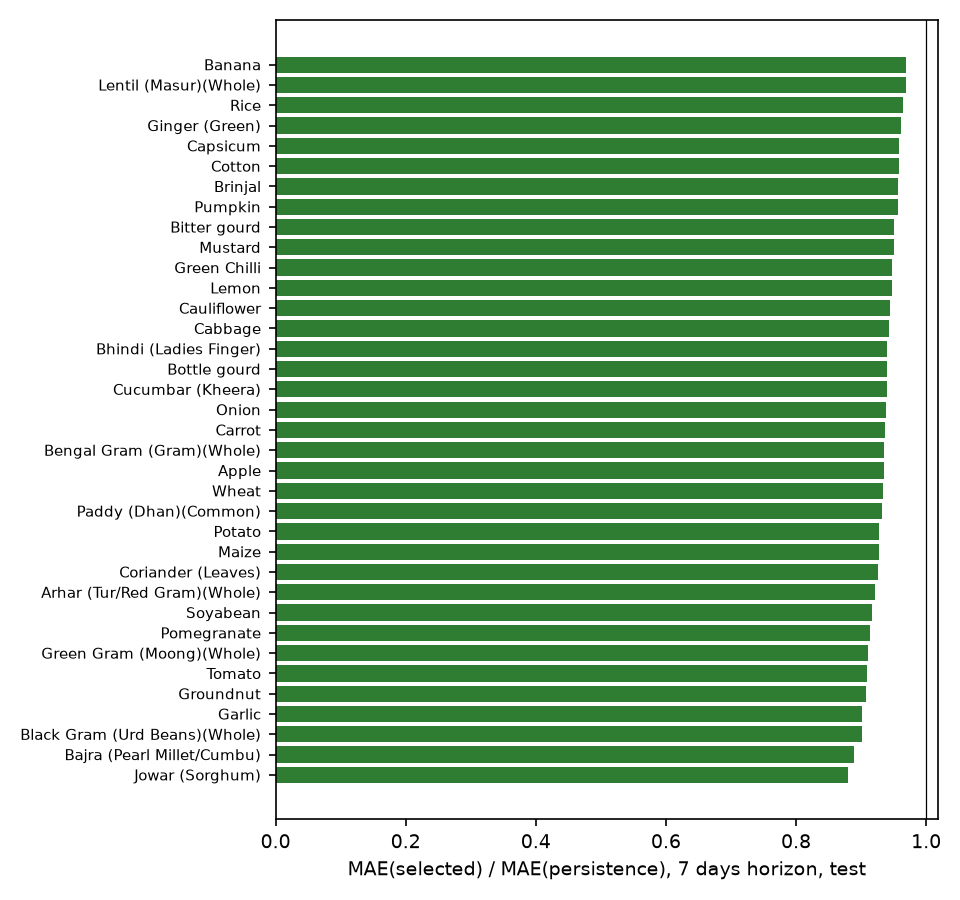
\includegraphics[width=0.62\linewidth]{rel_mae_by_commodity_h7.png}
\caption{Test MAE of the selected model relative to persistence, by commodity, at the 7-day horizon.}\label{fig:comm}
\end{figure}

\paragraph{A per-series statistical baseline.}
On a random sample of 400 panel series, we fitted simple exponential smoothing per series, with $\alpha$ chosen on training origins.
Its relative MAE (0.975 and 0.962 at the next-report and 3-day horizons) matches the global model on the same rows (0.976 and 0.960).
The global model is clearly better at 7 and 14 days (0.946 vs.\ 0.967, and 0.935 vs.\ 0.975).
\emph{At the shortest horizons, the advantage of machine learning over a well-tuned smoother is therefore nil.} It appears only once cross-market and seasonal information has time to matter.

\paragraph{Sub-periods.}
On the archive, relative MAE before the AGMARKNET~2.0 migration (2025-01 to 2025-10) is 0.970, 0.951, 0.937 and 0.922.
After it (2025-11 to 2026-04, only 4--6\% of test rows because the mirror is incomplete), the gains shrink to 0.993, 0.977, 0.968 and 0.944.
On complete official data the post-migration values are 0.976, 0.962, 0.962 and 0.937 (Section~\ref{sec:prospective}).

\paragraph{Ablation.}
For the 7-day GBT, removing any one of the calendar, level or seasonal feature groups changes the test relative MAE by at most 0.004 (from 0.944).
Removing the same-day cross-market features raises it to 0.960, and a returns-only model (three features) reaches 0.970.
The most important random-forest features at 7 days are the 7-day deviation (0.18), the last return (0.12) and the national and state cross-market deviations (0.10 and 0.09).
Information from other markets, not calendar or seasonality, is therefore what the models add over persistence.

\subsection{Prediction intervals}\label{sec:intervalresults}
Empirical test coverage of the nominal 80\% intervals is 78.6\%, 79.4\%, 80.0\% and 80.5\%; for the 90\% intervals it is 88.9--90.5\%.
Across volatility quintiles, coverage stays between 77.2\% and 82.0\% (Figure~\ref{fig:cov}).
Widths adapt strongly: the mean 80\% width runs from 2--8\% of the price in the calmest quintile to 45--88\% in the most volatile.
On the archive, 80\% coverage after the migration appeared to fall to 67.6--72.9\%.
Re-scoring the same frozen models on the complete official data, however, gives 78.0--78.7\% (Section~\ref{sec:prospective}).
The apparent loss of calibration was therefore largely an artefact of the mirror's missing reports, not a property of the intervals.
Adaptive conformal methods \cite{gibbs2021adaptive} remain the natural safeguard against genuine shift, but we did not implement them.

\begin{figure}[t]
\centering
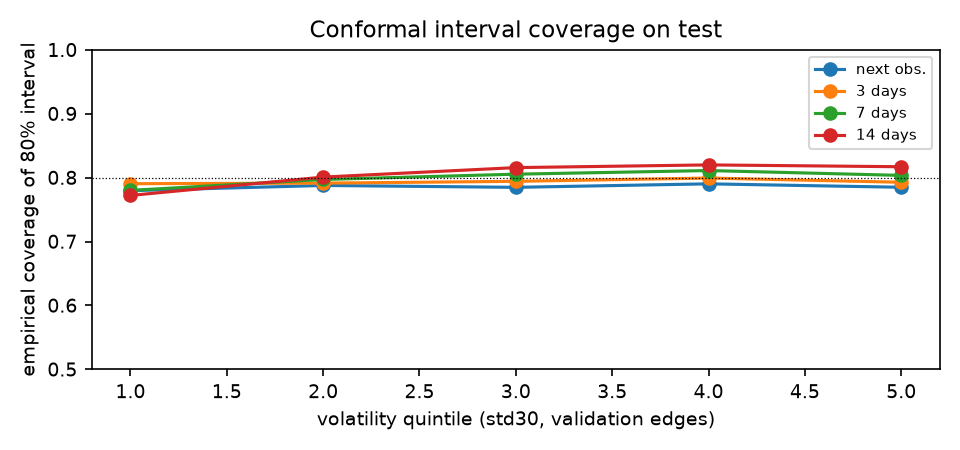
\includegraphics[width=0.7\linewidth]{interval_coverage.png}
\caption{Test coverage of 80\% split-conformal intervals by volatility quintile, with bin edges from validation.}\label{fig:cov}
\end{figure}

\subsection{Decision rule}\label{sec:decisions}
On the test period, the rule abstains (\textsc{watch}) on 97.8--98.5\% of report-days.
At 7 days:
\begin{itemize}
  \item \textsc{hold} fires on 0.5\% of report-days; the realised price beats today's price plus holding cost 80.0\% of the time;
  \item \textsc{sell} fires on 1.0\%; the realised price is below today's 67.8\% of the time.
\end{itemize}
The median realised 7-day change after \textsc{hold} is $+46.8\%$.
This reveals what the rule mostly detects: reports far below the series' recent level that subsequently revert.
Some of these may be reporting errors smaller than our factor-five sanity threshold.
These are hit rates on published modal prices, not farm-gate profits, and \textsc{compare} could not be back-tested because no transport data was available.

\subsection{Anomaly detection}
On 400k real test rows with 1\% injected corruptions, the production rule reaches PR-AUC 0.704 for any corruption.
This compares with 0.671 for a previous-report change score and 0.352 for the legacy commodity-IQR rule.
At its operating point, precision is 0.31, recall 0.85 and the false-positive rate 1.9\%.
For pure unit or keying errors the simple change score ranks best (PR-AUC 0.996).
Abrupt $\pm35$--60\% shocks are hard for every detector (best PR-AUC 0.25).
The rule flags 1.9\% of uncorrupted real rows; without labels we cannot say how many of these are genuine market events.

\subsection{Frozen models on complete and on new data}\label{sec:prospective}
After the main experiment, an API key for data.gov.in became available.
We back-filled \num{7.7}M official records for 2025-10-01 to 2026-10-22 and built a second silver layer (archive before October 2025, official data after).
We then scored the \emph{frozen} \texttt{fc\_main\_v3} models, conformal quantiles and MASE scales on it, with nothing refitted.

\paragraph{Test period, complete data.}
On the original test period re-scored with complete data (1.8--2.0M forecasts per horizon):
\begin{itemize}
  \item relative MAE is 0.972, 0.954, 0.943 and 0.925;
  \item 80\% coverage is 79.2--80.3\%;
  \item Diebold--Mariano $p\le3\times10^{-41}$.
\end{itemize}

\paragraph{Prospective period.}
On 2026-04-22 to 2026-10-22, six months that no model, tuning step or calibration had seen:
\begin{itemize}
  \item relative MAE is 0.963, 0.955, 0.958 and 0.952;
  \item 80\% coverage is 76.9--80.1\%;
  \item $p\le10^{-15}$;
  \item the models beat persistence on 59--67\% of series.
\end{itemize}
The 7- and 14-day gains are smaller than in the main test, which is consistent with models trained on data to 2023 ageing; retraining was not evaluated.

\subsection{Stability over time}\label{sec:systemsresults}
A rolling-origin backtest refits each horizon's selected configuration on expanding windows and tests on 2021, 2022, 2023 and 2024.
The resulting relative MAE ranges are:
\begin{itemize}
  \item next report: 0.970--0.976;
  \item 3 days: 0.952--0.960;
  \item 7 days: 0.936--0.946;
  \item 14 days: 0.920--0.936.
\end{itemize}
These bracket the main test values, so the improvement over persistence is not an artefact of one test year.
The 2024 fold coincides with the validation year.

\subsection{Streaming}
We replayed \num{20000} real archived reports through a six-partition Kafka topic at 2,000 events/s with labelled faults: 5\% duplicates, 2\% late re-sends, 1\% malformed messages, and local reordering.
Of \num{21524} messages:
\begin{itemize}
  \item \num{20000} distinct events reached silver, with none missing and none never sent;
  \item \num{1317} duplicate or late copies were removed by watermarked de-duplication;
  \item 207 malformed messages were quarantined;
  \item none were dropped by the watermark.
\end{itemize}
The canonicalised streaming rows matched the batch canonicalisation of the same records in all 14 compared columns, with 0 mismatches.
The median per-batch producer-to-sink latency was 1.7\,s with a 2\,s trigger.
The red-team review found that an earlier version let a malformed message advance the event-time watermark and silently discard every later event. Unusable messages are now quarantined before the watermark, and a regression test covers this case.

\subsection{Storage and distributed execution}
The silver layer (692\,MB, \num{1743} files) was loaded into a three-DataNode HDFS with replication 3.
fsck reported no missing or corrupt blocks, and a file remained readable, with an identical checksum, while a DataNode was stopped.
All DataNodes share one physical disk, and there is a single NameNode.
On a containerised standalone Spark cluster (2 workers, 6 cores, 1\,GB executors) reading from HDFS, the aggregation workload processed 11.3M real rows in 9.2\,s and the window-feature workload in 14.4\,s.
These runs exercise the distributed code path (separate driver and executor JVMs, network shuffle, HDFS reads) but not multi-machine scaling.

\subsection{Single-host scalability}
\begin{figure}[t]
\centering
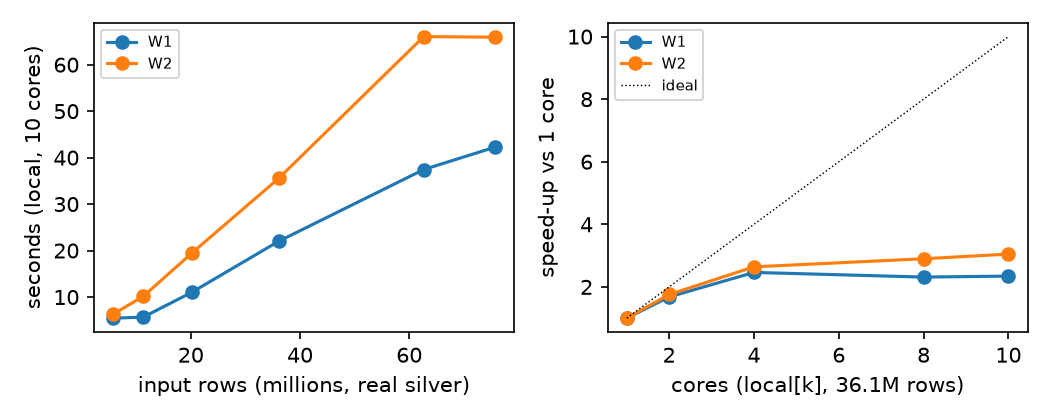
\includegraphics[width=0.9\linewidth]{scalability.png}
\caption{Left: run time against input size on the full silver layer (local mode, 10 cores). Right: speed-up against core count for 36.1M rows. W1 is an aggregation; W2 is per-entity window features.}\label{fig:scale}
\end{figure}
On one Apple M5 laptop (4 performance and 6 efficiency cores, 16\,GB), run time grows roughly linearly with input up to the full \num{75.6}M-row silver layer (Figure~\ref{fig:scale}).
Throughput is 1.6--2.0M rows/s for the aggregation and about 1.0M rows/s for the window features, with about 1\,GB of shuffle at full size and no disk spill.
Speed-up with cores flattens after four, matching the performance-core count: 2.5$\times$ for the aggregation and 3.0$\times$ for the window features at 10 cores.
The complete feature build for the forecasting panel (33M reports, 25 features, four targets) takes 8.3 minutes (\texttt{logs/f1\_build\_features.log}), and the full benchmark (38 model fits on 2M rows each, i.e.\ 32 candidates and 6 ablations, plus scoring of 6.4M test forecasts) takes 1\,h\,41\,min.


\subsection{Comparison with published results}\label{sec:comparison}
No published study we found uses daily mandi modal prices with these horizons, chronological purged splits and baselines.
We therefore quote prior numbers only as context.
\begin{itemize}
  \item Manogna et al.\ \cite{manogna2025deep} report a GRU MAPE of 14.59\% for onion and 10.58\% for tomato in their abstract, and 16.17\% and 14.81\% in the body.
    These come from an 80/20 hold-out of unclear horizon and aggregation. The authors explicitly chose not to use MASE, and we found no naive baseline in the sections we could read.
  \item Paul et al.\ \cite{paul2022brinjal} evaluate 17 Odisha markets for brinjal on a 90/10 split.
  \item Paul et al.\ \cite{paul2025deep} use monthly data.
\end{itemize}
Our WAPE of 5.6--11.1\% is not comparable with these MAPE figures: the denominators, horizons, aggregation and series differ.
The comparison we can defend is internal. On our data and splits, tuned learners beat persistence by 3--8\% in MAE, and beat a per-series smoother only beyond three days.
This is far smaller than the gains over ARIMA reported in the literature, for example GRU RMSEs four to six times lower than ARIMA's for onion and tomato in \cite{manogna2025deep}.
The difference suggests that the choice of baseline and protocol, rather than the choice of model, explains much of the spread in published results.
